% Options for packages loaded elsewhere
\PassOptionsToPackage{unicode}{hyperref}
\PassOptionsToPackage{hyphens}{url}
%
\documentclass[
]{article}
\usepackage{amsmath,amssymb}
\usepackage{lmodern}
\usepackage{iftex}
\ifPDFTeX
  \usepackage[T1]{fontenc}
  \usepackage[utf8]{inputenc}
  \usepackage{textcomp} % provide euro and other symbols
\else % if luatex or xetex
  \usepackage{unicode-math}
  \defaultfontfeatures{Scale=MatchLowercase}
  \defaultfontfeatures[\rmfamily]{Ligatures=TeX,Scale=1}
\fi
% Use upquote if available, for straight quotes in verbatim environments
\IfFileExists{upquote.sty}{\usepackage{upquote}}{}
\IfFileExists{microtype.sty}{% use microtype if available
  \usepackage[]{microtype}
  \UseMicrotypeSet[protrusion]{basicmath} % disable protrusion for tt fonts
}{}
\makeatletter
\@ifundefined{KOMAClassName}{% if non-KOMA class
  \IfFileExists{parskip.sty}{%
    \usepackage{parskip}
  }{% else
    \setlength{\parindent}{0pt}
    \setlength{\parskip}{6pt plus 2pt minus 1pt}}
}{% if KOMA class
  \KOMAoptions{parskip=half}}
\makeatother
\usepackage{xcolor}
\IfFileExists{xurl.sty}{\usepackage{xurl}}{} % add URL line breaks if available
\IfFileExists{bookmark.sty}{\usepackage{bookmark}}{\usepackage{hyperref}}
\hypersetup{
  pdftitle={Normal Distribution},
  pdfauthor={XDASI Fall 2021},
  hidelinks,
  pdfcreator={LaTeX via pandoc}}
\urlstyle{same} % disable monospaced font for URLs
\usepackage[margin=1in]{geometry}
\usepackage{color}
\usepackage{fancyvrb}
\newcommand{\VerbBar}{|}
\newcommand{\VERB}{\Verb[commandchars=\\\{\}]}
\DefineVerbatimEnvironment{Highlighting}{Verbatim}{commandchars=\\\{\}}
% Add ',fontsize=\small' for more characters per line
\usepackage{framed}
\definecolor{shadecolor}{RGB}{248,248,248}
\newenvironment{Shaded}{\begin{snugshade}}{\end{snugshade}}
\newcommand{\AlertTok}[1]{\textcolor[rgb]{0.94,0.16,0.16}{#1}}
\newcommand{\AnnotationTok}[1]{\textcolor[rgb]{0.56,0.35,0.01}{\textbf{\textit{#1}}}}
\newcommand{\AttributeTok}[1]{\textcolor[rgb]{0.77,0.63,0.00}{#1}}
\newcommand{\BaseNTok}[1]{\textcolor[rgb]{0.00,0.00,0.81}{#1}}
\newcommand{\BuiltInTok}[1]{#1}
\newcommand{\CharTok}[1]{\textcolor[rgb]{0.31,0.60,0.02}{#1}}
\newcommand{\CommentTok}[1]{\textcolor[rgb]{0.56,0.35,0.01}{\textit{#1}}}
\newcommand{\CommentVarTok}[1]{\textcolor[rgb]{0.56,0.35,0.01}{\textbf{\textit{#1}}}}
\newcommand{\ConstantTok}[1]{\textcolor[rgb]{0.00,0.00,0.00}{#1}}
\newcommand{\ControlFlowTok}[1]{\textcolor[rgb]{0.13,0.29,0.53}{\textbf{#1}}}
\newcommand{\DataTypeTok}[1]{\textcolor[rgb]{0.13,0.29,0.53}{#1}}
\newcommand{\DecValTok}[1]{\textcolor[rgb]{0.00,0.00,0.81}{#1}}
\newcommand{\DocumentationTok}[1]{\textcolor[rgb]{0.56,0.35,0.01}{\textbf{\textit{#1}}}}
\newcommand{\ErrorTok}[1]{\textcolor[rgb]{0.64,0.00,0.00}{\textbf{#1}}}
\newcommand{\ExtensionTok}[1]{#1}
\newcommand{\FloatTok}[1]{\textcolor[rgb]{0.00,0.00,0.81}{#1}}
\newcommand{\FunctionTok}[1]{\textcolor[rgb]{0.00,0.00,0.00}{#1}}
\newcommand{\ImportTok}[1]{#1}
\newcommand{\InformationTok}[1]{\textcolor[rgb]{0.56,0.35,0.01}{\textbf{\textit{#1}}}}
\newcommand{\KeywordTok}[1]{\textcolor[rgb]{0.13,0.29,0.53}{\textbf{#1}}}
\newcommand{\NormalTok}[1]{#1}
\newcommand{\OperatorTok}[1]{\textcolor[rgb]{0.81,0.36,0.00}{\textbf{#1}}}
\newcommand{\OtherTok}[1]{\textcolor[rgb]{0.56,0.35,0.01}{#1}}
\newcommand{\PreprocessorTok}[1]{\textcolor[rgb]{0.56,0.35,0.01}{\textit{#1}}}
\newcommand{\RegionMarkerTok}[1]{#1}
\newcommand{\SpecialCharTok}[1]{\textcolor[rgb]{0.00,0.00,0.00}{#1}}
\newcommand{\SpecialStringTok}[1]{\textcolor[rgb]{0.31,0.60,0.02}{#1}}
\newcommand{\StringTok}[1]{\textcolor[rgb]{0.31,0.60,0.02}{#1}}
\newcommand{\VariableTok}[1]{\textcolor[rgb]{0.00,0.00,0.00}{#1}}
\newcommand{\VerbatimStringTok}[1]{\textcolor[rgb]{0.31,0.60,0.02}{#1}}
\newcommand{\WarningTok}[1]{\textcolor[rgb]{0.56,0.35,0.01}{\textbf{\textit{#1}}}}
\usepackage{graphicx}
\makeatletter
\def\maxwidth{\ifdim\Gin@nat@width>\linewidth\linewidth\else\Gin@nat@width\fi}
\def\maxheight{\ifdim\Gin@nat@height>\textheight\textheight\else\Gin@nat@height\fi}
\makeatother
% Scale images if necessary, so that they will not overflow the page
% margins by default, and it is still possible to overwrite the defaults
% using explicit options in \includegraphics[width, height, ...]{}
\setkeys{Gin}{width=\maxwidth,height=\maxheight,keepaspectratio}
% Set default figure placement to htbp
\makeatletter
\def\fps@figure{htbp}
\makeatother
\setlength{\emergencystretch}{3em} % prevent overfull lines
\providecommand{\tightlist}{%
  \setlength{\itemsep}{0pt}\setlength{\parskip}{0pt}}
\setcounter{secnumdepth}{-\maxdimen} % remove section numbering
\ifLuaTeX
  \usepackage{selnolig}  % disable illegal ligatures
\fi

\title{Normal Distribution}
\author{XDASI Fall 2021}
\date{10/14/2021}

\begin{document}
\maketitle

{
\setcounter{tocdepth}{3}
\tableofcontents
}
\hypertarget{background}{%
\subsection{Background}\label{background}}

\begin{itemize}
\tightlist
\item
  \textbf{W\&S Chapter 10: Normal Distribution}
\end{itemize}

\hypertarget{additional-reading}{%
\subsubsection{Additional Reading}\label{additional-reading}}

\begin{itemize}
\tightlist
\item
  \href{https://xdas.bio.nyu.edu/references/Aho_Ch3.1-3.2_PDFs_Part1.pdf}{\textbf{Aho
  - Chapter 3.1-3.2: Probability Density Functions (Part 1)}}
\item
  \href{https://xdas.bio.nyu.edu/references/Aho_Ch_4.3_Statistics.pdf}{\textbf{Aho
  - Chapter 4.3: Statistics}}
\item
  \href{https://xdas.bio.nyu.edu/references/CalculusReview_2.0.pdf}{\textbf{Tranchina
  - Elements of Calculus}}
\end{itemize}

\hypertarget{normal-distribution}{%
\subsection{Normal distribution}\label{normal-distribution}}

The normal distribution is the most common distribution in statistics
and has many applications in biology. It is important because it
represents many processes in which the most likely outcome is the
average. Large sums of (small) random variables are often normally
distributed.

The Normal distribution is a \textbf{continuous} distribution with a
characteristic bell shape, the precise dimensions of which are governed
by its mean \(\mu\) and standard deviation \(\sigma\).

\begin{figure}
\centering
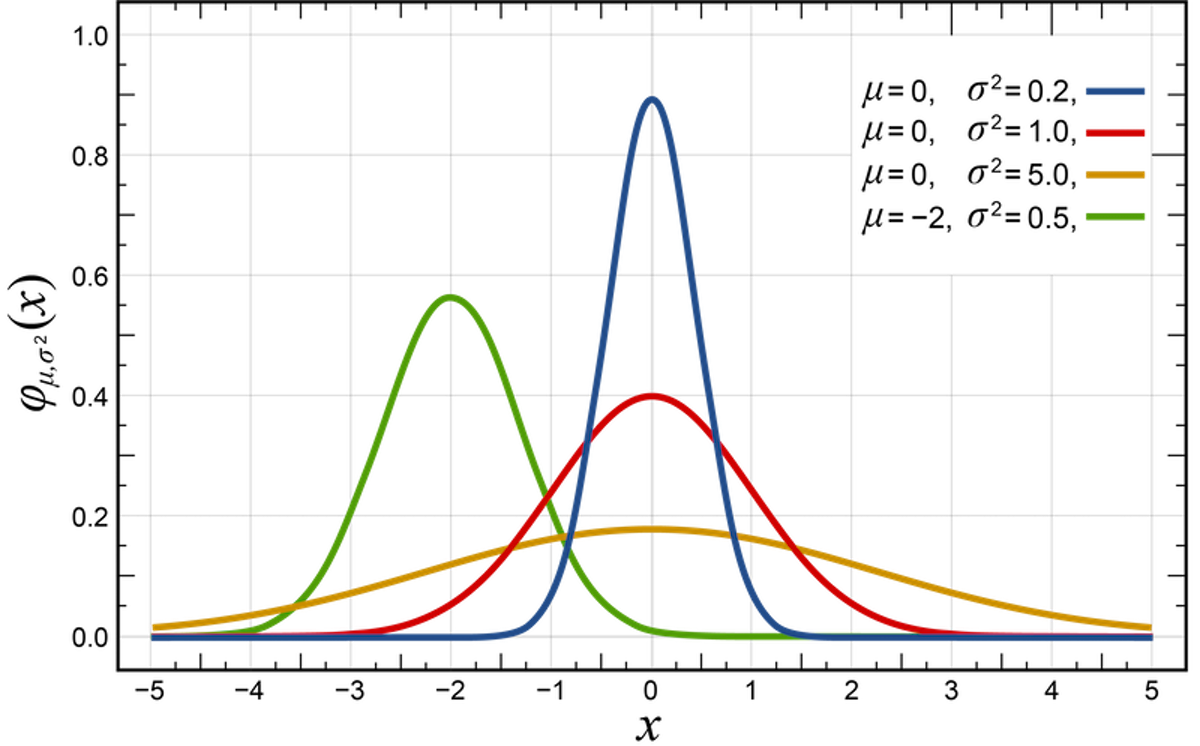
\includegraphics[width=0.5\textwidth,height=\textheight]{Images/Normal_Distribution_PDF.png}
\caption{Normal distributions with different mean and variance}
\end{figure}

Its mathematical description is:

PDF: \[ f(x) = \frac{1}{\sigma\sqrt{2\pi}} e^{-\frac{1}{2} 
               \left(\frac{x-\mu}{\sigma}\right)^2} \]

CDF: \[ F(x) = \int_{-\infty}^{\infty}
               \frac{1}{\sigma\sqrt{2\pi}} e^{-\frac{1}{2} 
               \left(\frac{x-\mu}{\sigma}\right)^2}dx = 1 \]

where:

\begin{enumerate}
\def\labelenumi{\arabic{enumi}.}
\tightlist
\item
  Outcomes \(x\) are continuous and independent.
\item
  \(x \in \mathbb{R}\)
\item
  \(\mu \in \mathbb{R}\)
\item
  \(\sigma > 0\)
\end{enumerate}

We write \(X\) \textasciitilde{} \(N(\mu,\sigma^2)\), where
\(E(X) = \mu\) and \(V(X) = \sigma^2\).

\hypertarget{standard-normal}{%
\subsection{Standard normal}\label{standard-normal}}

The standard normal distribution, or \emph{Z-distribution}, is a normal
or Gaussian distribution with \(\mu = 0\) and \(\sigma = 1\): \(Z\)
\textasciitilde{} \(N(0,1)\)

The normal distribution is standardized by subtracting the mean and
dividing over the SD: \[ Z = \frac{X - \mu}{\sigma}\]

Any outcome \(x_i\) from a normal distribution can be turned into a
\(z\)-score in the same maner.

As with any other distribution, we can ask questions like, ``What is the
chance of observing a value of \(x\) or less? \(x\) or more? between
\(x\) and \(y\)?''

We can also use the \textbf{inverse CDF}, or the
\textbf{\emph{quantile}} function, to find the value for some percentile
in the population (e.g.~the femur length that 80\% of the population is
under, which could be a factor in setting the seat pitch in airplanes).

\hypertarget{empirical-rule-for-the-standard-normal}{%
\paragraph{Empirical rule for the standard
normal}\label{empirical-rule-for-the-standard-normal}}

There is a general rule of thumb about how much of a distribution falls
within some number of standard deviations from the mean: a little over
2/3 of the data fall within 1SD, \textasciitilde95\% fall within 2SD,
and \textasciitilde99\% fall within 3SD.

\begin{figure}
\centering
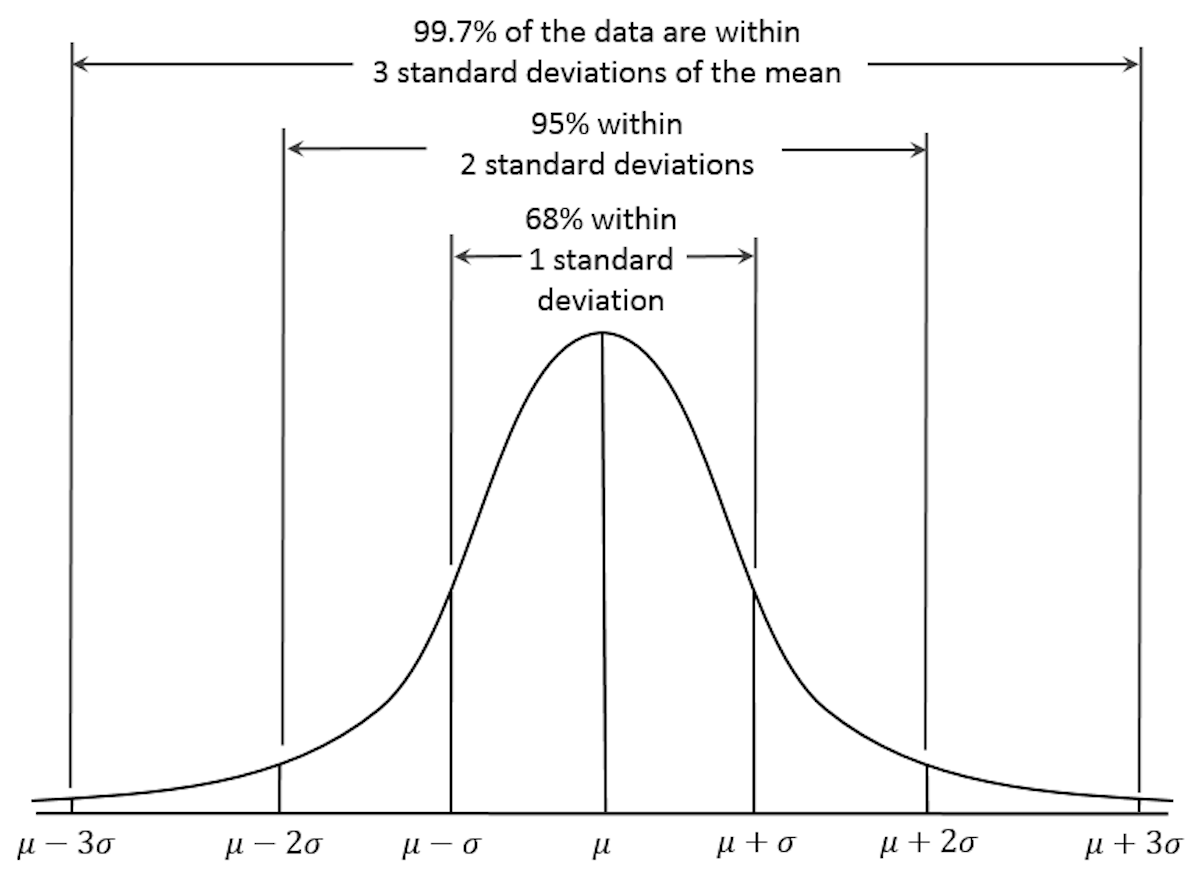
\includegraphics[width=0.6\textwidth,height=\textheight]{Images/Empirical_Rule.png}
\caption{Empirical rule for the normal distribution}
\end{figure}

If you were to sample any Normal distribution, it might look something
like the histogram here.

\begin{figure}
\centering
\includegraphics[width=0.5\textwidth,height=\textheight]{Images/Empirical_Rule_Histogram.png}
\caption{Sampling from the normal distribution}
\end{figure}

\hypertarget{what-controls-the-shape-of-the-distribution}{%
\paragraph{What controls the shape of the
distribution?}\label{what-controls-the-shape-of-the-distribution}}

\textbf{\emph{Bell-shaped curve}}: This is governed by the general
formula \(y = e^{-x^2}\). The height of this curve at \(x = 0\)
(i.e.~the y-intercept) is \(y = 1\).

\begin{figure}
\centering
\includegraphics[width=0.65\textwidth,height=\textheight]{Images/Exponential_Bell_Curve.png}
\caption{Exponential bell curve}
\end{figure}

The total area under the curve \(e^{-x^2}\) is:

\[ \int_{-\infty}^{\infty}e^{-x^2}dx = \sqrt{\pi} \approx 1.77\]

\textbf{\emph{Width and location of the curve}}: This is governed by the
value of the exponent. The Normal distribution is expressed in terms of
the mean, \(\mu\), and the variance, \(\sigma^2\), of the data.
Substituting the exponent with the term
\({-\frac{1}{2}\left(\frac{x-\mu}{\sigma}\right)^2}\) gives a curve that
is zero-centered around the mean \(\mu\) and has a standard deviation of
\(\sigma\).

\textbf{\emph{Area under the curve}}: In order to make the total
probability equal to one, we use a scaling factor (let's call this a
constant \(C\)) that is a multiplier of the exponential formula. This
constant turns out to be \(C = \frac{1}{\sigma\sqrt{2\pi}}\).

Deriving these equations is not trivial. We end up with the magical
number \(\pi\) in the equation because it turns out that using a polar
coordinate system, instead of Cartesian coordinates, is more natural to
describe this shape. If you want to get an idea of how the Normal PDF is
derived, check out this video on YouTube:
\href{https://www.youtube.com/watch?v=ebewBjZmZTw}{\textbf{Quick
derivation of the Normal PDF (4'50'')}}
(\url{https://www.youtube.com/watch?v=ebewBjZmZTw}).

\hypertarget{central-limit-theorem}{%
\subsection{Central limit theorem}\label{central-limit-theorem}}

The sampling distribution of sample means follows a normal distribution,
making the normal distribution extremely useful for learning the
properties of random samples. We covered the CLT in a previous class
(see link to class notes above).

\hypertarget{normal-approximation-of-the-binomial}{%
\subsection{Normal approximation of the
binomial}\label{normal-approximation-of-the-binomial}}

When the sample size is large, and \(p \approx 0.5\) (not too large or
too small), the normal distribution is a very good approximation to the
binomial.

\hypertarget{example}{%
\subsection{Example}\label{example}}

The average weight of an adult female greyhound is 63 pounds, with a
standard deviation of 8 pounds. What proportion of female greyhounds
weigh less than or equal to 55 pounds?

\begin{Shaded}
\begin{Highlighting}[]
\FunctionTok{pnorm}\NormalTok{(}\DecValTok{55}\NormalTok{, }\AttributeTok{mean =} \DecValTok{63}\NormalTok{, }\AttributeTok{sd =} \DecValTok{8}\NormalTok{)}
\end{Highlighting}
\end{Shaded}

\begin{verbatim}
## [1] 0.1586553
\end{verbatim}

What proportion weigh between 60 and 65 pounds?

\[ P(60 \le X \le 65) = \int_{60}^{65}f(x)dx =\Big[ F(x) \Big]_{60}^{65}  \\
= \int_{-\infty}^{65}f(x)dx -  
               \int_{-\infty}^{60}f(x)dx = F(65) - F(60)  \]

\begin{Shaded}
\begin{Highlighting}[]
\CommentTok{\# note that you cannot use the summation method for a continuous distribution;}
\CommentTok{\# you have to subtract CDF up to each point to get the probability for the interval}
\FunctionTok{pnorm}\NormalTok{(}\DecValTok{65}\NormalTok{, }\AttributeTok{mean =} \DecValTok{63}\NormalTok{, }\AttributeTok{sd =} \DecValTok{8}\NormalTok{) }\SpecialCharTok{{-}} \FunctionTok{pnorm}\NormalTok{(}\DecValTok{60}\NormalTok{, }\AttributeTok{mean =} \DecValTok{63}\NormalTok{, }\AttributeTok{sd =} \DecValTok{8}\NormalTok{)}
\end{Highlighting}
\end{Shaded}

\begin{verbatim}
## [1] 0.2448761
\end{verbatim}

It can safely be said that 75\% weigh no more than what amount? This is
a question that calls for the quantile function (inverse CDF):

\begin{Shaded}
\begin{Highlighting}[]
\FunctionTok{qnorm}\NormalTok{(}\FloatTok{0.75}\NormalTok{, }\AttributeTok{mean =} \DecValTok{63}\NormalTok{, }\AttributeTok{sd =} \DecValTok{8}\NormalTok{)}
\end{Highlighting}
\end{Shaded}

\begin{verbatim}
## [1] 68.39592
\end{verbatim}

\end{document}
